% Hacker: MeanFlow. CS 2883R, Wed 14 Oct 2026. Juntang Wang.
% Design draft: results are TBD boxes. Budget 5:00; timing above each frame.
% Build: latexmk -pdf main.tex
\documentclass[aspectratio=169,12pt]{beamer}
\usetheme[progressbar=none, numbering=counter]{moloch}

\usepackage[sfdefault,light]{FiraSans}
\usepackage{inconsolata}
\usepackage[T1]{fontenc}
\usepackage{listings}
\usepackage{tikz}
\usepackage{qrcode}
\usepackage{booktabs}
\usepackage[authoryear, round]{natbib}
\definecolor{cite}{HTML}{1F5FBF}  % citations and URLs: blue, clickable
\hypersetup{colorlinks=true, citecolor=cite, urlcolor=cite, linkcolor=.}
\renewcommand{\bibsection}{}                          % the frame title is enough
\setbeamertemplate{frametitle continuation}{}         % no "i, ii" on split frames
\bibliographystyle{plainnat}
% gray (Author, year) after a dataset name
\newcommand{\src}[1]{{\scriptsize\color{mute}\citep{#1}}}

\definecolor{ink}{HTML}{222222}
\definecolor{mute}{HTML}{8a8a8a}     % Flow Matching
\definecolor{mf}{HTML}{e8710a}       % MeanFlow
\definecolor{crimson}{HTML}{A51C30}  % Harvard; title slide only

\setbeamercolor{normal text}{fg=ink, bg=white}
\setbeamercolor{frametitle}{fg=ink, bg=white}
\setbeamercolor{page number in head/foot}{fg=mute}
\setbeamertemplate{itemize items}{\color{mute}--}

% code: faint panel; jvp (the one key op) in MeanFlow orange; other calls bold
\lstset{language=Python, basicstyle=\ttfamily\scriptsize\color{ink},
  columns=fullflexible, keepspaces=true, showstringspaces=false,
  numbers=left, numberstyle=\tiny\color{mute}, numbersep=8pt, xleftmargin=1.4em,
  backgroundcolor=\color{black!4}, frame=single, rulecolor=\color{black!4},
  framesep=4pt, aboveskip=2pt, belowskip=0pt,
  keywordstyle=\color{ink}\bfseries, commentstyle=\color{mute}\itshape,
  emph={[1]jvp}, emphstyle={[1]\color{mf}\bfseries},
  emph={[2]sample_t_r, randn_like, stopgrad, metric, adaptive_l2_loss, model},
  emphstyle={[2]\bfseries}}

% \tbd{width}{height}{label}: a result not produced yet
\newcommand{\tbd}[3]{%
  \tikz\node[draw=mf!60, dashed, minimum width=#1, minimum height=#2,
    text width=#1-6mm, align=center, font=\scriptsize, text=mute,
    execute at begin node={\hyphenpenalty=10000}]{#3};}
\newcommand{\TBD}{{\color{mf}TBD}}
% Data slide: a group header row spanning the table
\newcommand{\datahead}[1]{%
  \multicolumn{4}{@{}l}{\rule{0pt}{14pt}\bfseries #1} \\}
% listings number styles for slide 2: row 6 is haidog's extra forward pass,
% shown as "+" there and left blank in Alg. 1; later rows are renumbered n-1
\newcommand{\rownum}[2]{\ifnum#2<6 #2\else\ifnum#2=6 #1\else\the\numexpr#2-1\relax\fi\fi}
\newcommand{\gapnum}[1]{\rownum{}{#1}}
\newcommand{\plusnum}[1]{\rownum{\color{mf}+}{#1}}
\newcommand{\lab}[1]{\\[3pt]{\scriptsize #1}}
% Results slides: fixed-width, vertically centred row label, so both grids align
\newcommand{\rowlab}[1]{\raisebox{0.9cm}{\makebox[1.9cm][r]{#1}}}
\newcommand{\pan}[1]{\includegraphics[width=1.85cm,height=1.85cm]{#1}}            % one model panel
\newcommand{\cls}[1]{\makebox[1.05cm]{\includegraphics[height=1.85cm]{#1}}}      % one class, two samples

% Colab link, branch TBD. \_ escaped for qrcode.
\newcommand{\colabqr}{https://colab.research.google.com/github/qqgjyx/CS-2883R/blob/main/2026-10-14\_meanflow/meanflow.ipynb}

\newsavebox{\titleinfo}
\newlength{\titleinfoht}

\begin{document}

% 1. Title (0:15). Subtitle = the role's asks: core code, toy, demo.
% Grid: one left edge; QR spans exactly the info block below the rule.
\begin{frame}[plain]
  \sbox{\titleinfo}{\begin{minipage}[b]{0.7\textwidth}
    Juntang Wang $\cdot$ {\color{mf}Hacker}\\[2pt]
    {\small\color{crimson} Harvard CS 2883R $\cdot$ 14 Oct 2026}\\[10pt]
    {\scriptsize\color{mute} Zhengyang Geng, Mingyang Deng, Xingjian Bai, J.~Zico Kolter, Kaiming He.\\
      Mean Flows for One-step Generative Modeling. arXiv 2505.13447}
  \end{minipage}}%
  \settototalheight{\titleinfoht}{\usebox{\titleinfo}}%
  \vfill
  {\LARGE\bfseries MeanFlow, from scratch}\\[6pt]
  {\large Learn the average, not the instant}\hfill
    {\scriptsize\color{mute} scan, then Run all in Colab}\\[-4pt]
  \textcolor{crimson}{\rule{\textwidth}{0.8pt}}\\[8pt]
  \usebox{\titleinfo}\hfill
  {\hypersetup{urlcolor=black}% clickable, but black, not link-blue
   \raisebox{\depth}{\qrcode[height=\titleinfoht]{\colabqr}}}% qrcode is centred on the baseline
  \vfill
\end{frame}

% 2. The method (1:00): symbols drawn on top, paper vs mine below
\begin{frame}[fragile]{Method, as implemented}
  % the paper's Fig. 3, full (vector, from the arXiv source)
  \centering
  \begin{tikzpicture}
    \node[inner sep=0pt] (fig) {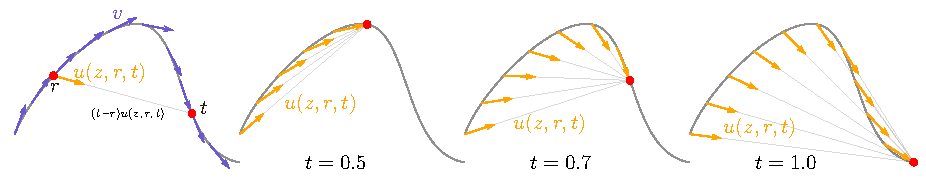
\includegraphics[height=2.4cm]{figs/paper_fig3.pdf}};
    \node[anchor=north east, inner sep=0pt, font=\tiny, text=mute] at (fig.north east)
      {\citet{geng2025meanflow}, Fig.~3};
  \end{tikzpicture}
  \vfill
  % paper Alg. 1 vs haidog-yaqub/MeanFlow meanflow.py, mode "meanflow" (lines 141-211, abridged)
  \begin{columns}[t]
    \column{0.40\textwidth}
      {\scriptsize\color{mute} paper, Alg.~1}
% row 6 left blank, level with haidog's extra forward pass
\begin{lstlisting}[numberstyle=\tiny\color{mute}\gapnum]
t, r = sample_t_r()
e = randn_like(x)
z = (1 - t) * x + t * e
v = e - x
u, dudt = jvp(fn, (z, r, t), (v, 0, 1))

u_tgt = v - (t - r) * dudt
error = u - stopgrad(u_tgt)
loss = metric(error)
\end{lstlisting}
    \column{0.56\textwidth}
      {\scriptsize\color{mute} ours, \texttt{meanflow.py} (abridged)$^1$}
\begin{lstlisting}[numberstyle=\tiny\color{mute}\plusnum]
t, r, w = self.sample_t_r(batch_size, device)
e = torch.randn_like(x)
z = (1 - t_) * x + t_ * e
v = e - x
_, dudt = jvp(model, (z, t, r), (v_c, 1, 0))
u_p, v_p = model(z, t, r)
u_tgt = v_hat - (t_ - r_) * dudt
mf_loss = adaptive_l2_loss(u_p - stopgrad(u_tgt))
return mf_loss + fm_loss
\end{lstlisting}
      {\tiny\color{mute}
        \texttt{v\_c}: the model's own $v$ head, not $e - x$; \texttt{fm\_loss} trains it\\
        \texttt{v\_hat} $= v + (1 - 1/w)(v_c - v_{uc})$: $v$ with CFG folded in\\
        $^1$adapted from \href{https://github.com/haidog-yaqub/MeanFlow}{\texttt{github.com/haidog-yaqub/MeanFlow}}\par}
  \end{columns}
\end{frame}

% 3. Data (0:20)
\begin{frame}{Data}
  \centering\footnotesize
  \renewcommand{\arraystretch}{1.15}\setlength{\tabcolsep}{5pt}
  % n = training set size; d = one sample's shape, channels x height x width
  \begin{tabular}{@{}lrll@{}}
    \toprule
    dataset & $n$ & $d$ & what \\
    \midrule
    \datahead{Synthetic}
    checkerboard \src{grathwohl2019ffjord} & $\infty$ & $2$ & point on 8 squares \\
    Swiss roll \src{sohl2015deep}          & $\infty$ & $2$ & point on a thin spiral \\
    \datahead{Real-world}
    MNIST \src{lecun1998gradient}          & 60{,}000 & $1{\times}28{\times}28$ & digit, 10 classes \\
    Fashion-MNIST \src{xiao2017fashion}    & 60{,}000 & $1{\times}28{\times}28$ & clothing, 10 classes \\
    \datahead{Real-world, big$^1$}
    ImageNet \src{deng2009imagenet}        & 1{,}281{,}167 & $3{\times}256{\times}256$ & photo, 1000 classes \\
    \bottomrule
  \end{tabular}\\[6pt]
  \begin{minipage}{\linewidth}\raggedright\tiny\color{mute}
    $^1$training configuration: MF-XL/2, 240 epochs, batch 256,
    $4{\times}32{\times}32$ VAE latents, 8$\times$H100. The other datasets: a single RTX 5080 / Colab
  \end{minipage}
\end{frame}

% 4. Results, synthetic (0:30): rows = datasets, columns = models. Flow Matching at
% several step counts (the v head, integrated) against MeanFlow in one step (the u head)
\begin{frame}{Results}
  \centering\scriptsize
  \setlength{\tabcolsep}{2pt}
  \begin{tabular}{@{}r*{6}{c}@{}}
    & data & {\color{mute}FM, 1 step} & {\color{mute}FM, 2} & {\color{mute}FM, 4}
      & {\color{mute}FM, 50} & {\color{mf}MeanFlow, 1 step} \\
    \rowlab{checkerboard} & \pan{figs/r_checkerboard_data.png} & \pan{figs/r_checkerboard_fm1.png} & \pan{figs/r_checkerboard_fm2.png} & \pan{figs/r_checkerboard_fm4.png} & \pan{figs/r_checkerboard_fm50.png} & \pan{figs/r_checkerboard_mf1.png} \\
    \rowlab{Swiss roll} & \pan{figs/r_swissroll_data.png} & \pan{figs/r_swissroll_fm1.png} & \pan{figs/r_swissroll_fm2.png} & \pan{figs/r_swissroll_fm4.png} & \pan{figs/r_swissroll_fm50.png} & \pan{figs/r_swissroll_mf1.png} \\
  \end{tabular}\\[6pt]
  {\color{mute} same starting noise in every panel; FM = the $v$ head, integrated}
\end{frame}

% 5. Results, real-world (0:30): same grid; rows = datasets, columns = classes.
% Ten class cells span the width of the six model cells above; two samples per cell.
\begin{frame}{Results (contd.)}
  \centering\scriptsize
  \setlength{\tabcolsep}{2pt}
  \begin{tabular}{@{}r*{10}{c}@{}}
    & 0 & 1 & 2 & 3 & 4 & 5 & 6 & 7 & 8 & 9 \\
    \rowlab{MNIST} & \cls{figs/c_mnist_0.png} & \cls{figs/c_mnist_1.png} & \cls{figs/c_mnist_2.png} & \cls{figs/c_mnist_3.png} & \cls{figs/c_mnist_4.png} & \cls{figs/c_mnist_5.png} & \cls{figs/c_mnist_6.png} & \cls{figs/c_mnist_7.png} & \cls{figs/c_mnist_8.png} & \cls{figs/c_mnist_9.png} \\
    \rowlab{Fashion-MNIST} & \cls{figs/c_fashion_0.png} & \cls{figs/c_fashion_1.png} & \cls{figs/c_fashion_2.png} & \cls{figs/c_fashion_3.png} & \cls{figs/c_fashion_4.png} & \cls{figs/c_fashion_5.png} & \cls{figs/c_fashion_6.png} & \cls{figs/c_fashion_7.png} & \cls{figs/c_fashion_8.png} & \cls{figs/c_fashion_9.png} \\
  \end{tabular}\\[6pt]
  {\color{mf}MeanFlow}{\color{mute}, 1 step, two samples per class}\\
  {\color{mute}Fashion: T-shirt, trouser, pullover, dress, coat, sandal, shirt, sneaker, bag, ankle boot}
\end{frame}

% 5. The chord: the core mechanism (0:45). One network, two heads, same noise:
% the v head integrated over 100 small steps traces the path; the u head jumps once.
\begin{frame}{The jump is the average of the path}
  \begin{columns}[t]
    \column{0.5\textwidth}
      \centering
      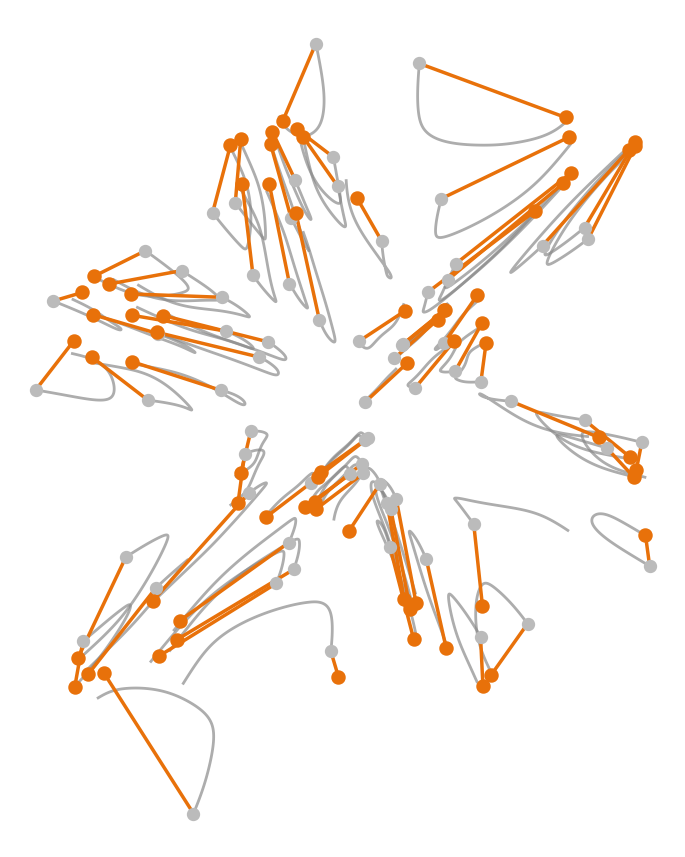
\includegraphics[height=4.2cm]{figs/j_checkerboard.png}\\[2pt]
      {\scriptsize {\color{mute}$v$ head, 100 steps} vs {\color{mf}$u$ head, 1 jump}}\\
      {\small jump vs path end: \textbf{0.08}} {\scriptsize\color{mute}(shuffled 4.34)}
    \column{0.46\textwidth}
      \centering
      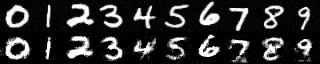
\includegraphics[width=\linewidth]{figs/j_mnist.png}\\[2pt]
      {\scriptsize top {\color{mute}$v$ head, 100 steps} $\cdot$ bottom {\color{mf}$u$ head, 1 step}}\\
      {\small per-pixel gap: \textbf{0.08}} {\scriptsize\color{mute}(shuffled 0.21)}\\[10pt]
      {\small $u = \frac{1}{t-r}\int_r^t v\,d\tau$}\\[4pt]
      {\scriptsize\color{mute} one network, two heads, same starting noise}
  \end{columns}
\end{frame}

% 6. Break the tangent (0:40)
\begin{frame}{Break the JVP, break the jump}
  \centering\vfill
  \begin{minipage}[t]{0.24\textwidth}\centering
    
\includegraphics[width=3.3cm]{figs/a_t1_r0.png}\lab{{\color{mf}$(v,0,1)$, correct}\\{\color{mute}paper FID 61 $\cdot$ ours 0.65}}\end{minipage}\hfill
  \begin{minipage}[t]{0.24\textwidth}\centering
    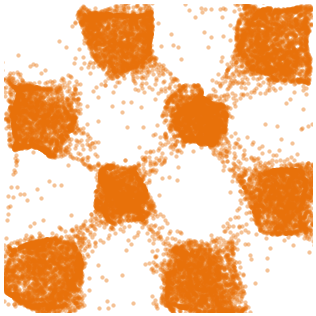
\includegraphics[width=3.3cm]{figs/a_t1_r1.png}\lab{$(v,1,1)$\\{\color{mute}paper FID 138 $\cdot$ ours 0.60}}\end{minipage}\hfill
  \begin{minipage}[t]{0.24\textwidth}\centering
    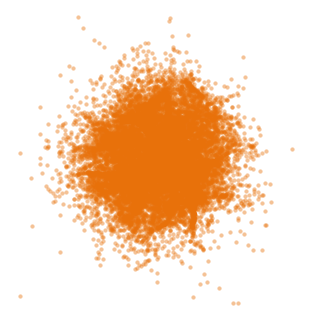
\includegraphics[width=3.3cm]{figs/a_t0_r0.png}\lab{$(v,0,0)$\\{\color{mute}paper FID 268 $\cdot$ ours 0.24}}\end{minipage}\hfill
  \begin{minipage}[t]{0.24\textwidth}\centering
    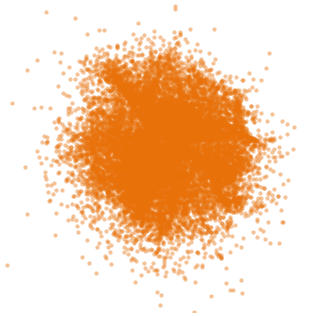
\includegraphics[width=3.3cm]{figs/a_t0_r1.png}\lab{$(v,1,0)$\\{\color{mute}paper FID 329 $\cdot$ ours 0.29}}\end{minipage}\\[12pt]
  {\scriptsize\color{mute} JVP tangent for $(\partial_z u, \partial_r u, \partial_t u)$\\
    paper: Tab.~1b, ImageNet FID $\downarrow$ $\cdot$ ours: checkerboard overlap $\uparrow$ $\cdot$ same order except the two worst}
  \vfill
\end{frame}

% 8. Closer (0:30): the cat, then flip to the Colab tab to show the live run finished
\begin{frame}[plain]
  \centering\vfill
  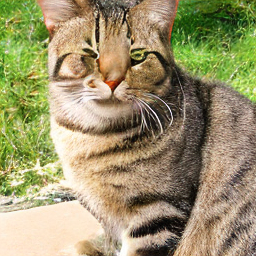
\includegraphics[height=4.2cm]{figs/cat.png}\\[16pt]
  {\Large Thank you}\\[6pt]
  {\scriptsize\color{mute} one MeanFlow step, ImageNet class 281 (tabby), 1 of 8 seeds; model by zhuyu-cs/MeanFlow}\\[14pt]
  {\small\color{mf} $\rightarrow$ back to Colab: the live run}
  \vfill
\end{frame}

% ---------- backup ----------
\appendix

\begin{frame}{Setup}
  \centering\scriptsize
  \renewcommand{\arraystretch}{1.15}\setlength{\tabcolsep}{5pt}
  % synthetic points are reshaped to 1x1x2 "images" so the same code runs them
  \begin{tabular}{@{}llll@{}}
    \toprule
    & \bfseries Synthetic & \bfseries Real-world & \bfseries Real-world, big \\
    \midrule
    code         & ours                                & ours                                  & zhuyu-cs \\
    network      & MLP $5{\times}512$, Fourier $z$ & DiT, 4 layers, width 192 & DiT-XL/2, 28 layers \\
    input        & $1{\times}1{\times}2$ (2D point, reshaped) & $1{\times}32{\times}32$         & $4{\times}32{\times}32$ latent \\
    params       & 1.1M                                & 3.1M, patch $4{\times}4$              & 677M, patch $2{\times}2$ \\
    loss         & \texttt{meanflow} mode, $p = 0.75$  & \texttt{meanflow} mode, $p = 1$       & MeanFlow + CFG \\
    $t, r$ sampler & logit-normal$(-2, 2)$             & logit-normal$(-0.4, 1)$               & --- \\
    JVP          & \multicolumn{2}{l}{\texttt{torch.func.jvp}, tangent from the $v$ head} & --- \\
    CFG          & none                                & $w \in [1, 7.5]$, sampled at 4.25     & folded in \\
    optimizer    & \multicolumn{2}{l}{AdamW, lr $10^{-3}$, cosine; batch 1024 / 128}         & batch 256 \\
    training     & 20{,}000 steps                      & 3{,}000 steps                         & 240 epochs \\
    time         & 94\,s each (RTX 5080)               & 131\,s each (RTX 5080)                & 8$\times$H100 \\
    \bottomrule
  \end{tabular}
\end{frame}

\begin{frame}[allowframebreaks]{References}
  \scriptsize
  \bibliography{refs}
\end{frame}

\end{document}
